\documentclass[aspectratio=169, 11pt]{beamer}

% ============================================================
% THEME BASE
% ============================================================
\usetheme{Madrid}
\usecolortheme{whale}

% ============================================================
% PACKAGES
% ============================================================
\usepackage[T1]{fontenc}
\usepackage[utf8]{inputenc}
\usepackage{graphicx}
\usepackage{booktabs}
\usepackage{tikz}
\usepackage{pgfplots}
\usepackage{amsmath}
\usepackage{hyperref}
\usepackage{multicol}
\usepackage{xcolor}

% ============================================================
% TIKZ LIBRARIES
% ============================================================
\usetikzlibrary{arrows.meta, positioning, shapes.geometric, calc, decorations.pathmorphing}

% ============================================================
% PGFPLOTS COMPATIBILITY
% ============================================================
\pgfplotsset{compat=1.18}

% ============================================================
% COLOR DEFINITIONS (Fintech V4 Palette)
% ============================================================
\definecolor{MLPURPLE}{HTML}{9467BD}
\definecolor{MLBLUE}{HTML}{1F77B4}
\definecolor{MLRED}{HTML}{D62728}
\definecolor{MLORANGE}{HTML}{FF7F0E}
\definecolor{MLGREEN}{HTML}{2CA02C}
\definecolor{MLGRAY}{HTML}{7F7F7F}
\definecolor{MLTEAL}{HTML}{0D7377}
\definecolor{MLCYAN}{HTML}{14BDEB}

% Lowercase aliases for use in \textcolor{}
\colorlet{mlpurple}{MLPURPLE}
\colorlet{mlblue}{MLBLUE}
\colorlet{mlred}{MLRED}
\colorlet{mlorange}{MLORANGE}
\colorlet{mlgreen}{MLGREEN}
\colorlet{mlgray}{MLGRAY}
\colorlet{mlteal}{MLTEAL}
\colorlet{mlcyan}{MLCYAN}

% ============================================================
% BEAMER COLOR CUSTOMIZATION
% ============================================================
\setbeamercolor{structure}{fg=MLTEAL}
\setbeamercolor{palette primary}{bg=MLTEAL, fg=white}
\setbeamercolor{palette secondary}{bg=MLTEAL!80, fg=white}
\setbeamercolor{palette tertiary}{bg=MLTEAL!60, fg=white}
\setbeamercolor{palette quaternary}{bg=MLTEAL!40, fg=white}
\setbeamercolor{frametitle}{bg=MLTEAL!10, fg=MLTEAL}
\setbeamercolor{frametitle right}{bg=MLTEAL!5}
\setbeamercolor{block title}{bg=MLTEAL, fg=white}
\setbeamercolor{block body}{bg=MLTEAL!8, fg=black}
\setbeamercolor{block title alerted}{bg=MLRED, fg=white}
\setbeamercolor{block body alerted}{bg=MLRED!8, fg=black}
\setbeamercolor{block title example}{bg=MLGREEN, fg=white}
\setbeamercolor{block body example}{bg=MLGREEN!8, fg=black}
\setbeamercolor{title}{fg=white}
\setbeamercolor{subtitle}{fg=MLCYAN}
\setbeamercolor{author}{fg=white}
\setbeamercolor{institute}{fg=white}
\setbeamercolor{date}{fg=white}
\setbeamercolor{title page header}{bg=MLTEAL}

% ============================================================
% NAVIGATION AND FOOTLINE
% ============================================================
\setbeamertemplate{navigation symbols}{}

\setbeamertemplate{footline}{%
  \leavevmode%
  \hbox{%
    \begin{beamercolorbox}[wd=.333\paperwidth, ht=2.25ex, dp=1ex, center]{palette primary}%
      \usebeamerfont{author in head/foot}\insertshortauthor
    \end{beamercolorbox}%
    \begin{beamercolorbox}[wd=.334\paperwidth, ht=2.25ex, dp=1ex, center]{palette secondary}%
      \usebeamerfont{title in head/foot}\insertshorttitle
    \end{beamercolorbox}%
    \begin{beamercolorbox}[wd=.333\paperwidth, ht=2.25ex, dp=1ex, right]{palette tertiary}%
      \usebeamerfont{date in head/foot}%
      \insertframenumber{} / \inserttotalframenumber\hspace*{2ex}
    \end{beamercolorbox}%
  }%
  \vskip0pt%
}

% ============================================================
% BOTTOM NOTE COMMAND
% ============================================================
\newcommand{\bottomnote}[1]{%
  \vfill
  \begin{beamercolorbox}[wd=\textwidth, ht=2ex, dp=1ex]{palette primary}%
    \tiny\hspace{1em}#1
  \end{beamercolorbox}%
}

% ============================================================
% GRAPHICS PATH
% ============================================================
\graphicspath{{figures/}}

% ============================================================
% COURSE METADATA
% ============================================================
\title{Financial Technology (FinTech)}
\author{Joerg Osterrieder}
\institute{University of Zurich \\ Department of Finance}
\date{Spring 2026}


% ============================================================
% L01 OVERVIEW VARIANT  (~26 frames)
% Variant 2 of 6 -- Three-zone architecture: INTRO / CORE / CLOSING
% Framework: PMSP (Problem -- Method -- Solution -- Practice)
% Audience: MSc Finance/Business, no coding assumed
% ============================================================

\subtitle{Understanding the Revolution in Financial Services}

% Short versions for footline
\title[Fintech: Foundations]{Financial Technology (FinTech) -- Lecture 1}
\author[J.\ Osterrieder]{Joerg Osterrieder}

\begin{document}

% ============================================================
% ZONE 1: INTRO
% Frames 1-5 -- Open, motivate, orient
% ============================================================

\section{Introduction}

% ---------------------------------------------------------
% Frame 1: Title Page
% ---------------------------------------------------------
\begin{frame}
  \titlepage
  \bottomnote{Lecture 1 of 7 $\cdot$ Financial Technology (FinTech) $\cdot$ MSc Programme $\cdot$ Spring 2026}
\end{frame}

% ---------------------------------------------------------
% Frame 2: Opening Cartoon
% ---------------------------------------------------------
\begin{frame}{The Revolution Started in a Garage}
  \begin{center}
    \includegraphics[width=0.90\textwidth]{figures/11_opening_cartoon/cartoon.pdf}
  \end{center}
  \bottomnote{This tension -- speed vs.\ scale, innovation vs.\ regulation -- is the heartbeat of this entire course.}
\end{frame}

% ---------------------------------------------------------
% Frame 3: Learning Objectives
% ---------------------------------------------------------
\begin{frame}{Learning Objectives}
  \begin{enumerate}
    \item \textbf{Describe} the defining characteristics of fintech and trace its historical evolution
          from early electronic banking to modern embedded finance. \textcolor{mlgray}{\small[Understand]}
    \item \textbf{Explain} how the 2008 financial crisis acted as a catalyst by eroding trust in
          traditional institutions. \textcolor{mlgray}{\small[Understand]}
    \item \textbf{Classify} the major collaboration models between banks and fintech companies.
          \textcolor{mlgray}{\small[Apply]}
    \item \textbf{Compare} the competitive advantages of incumbent banks vs.\ fintech startups.
          \textcolor{mlgray}{\small[Analyze]}
    \item \textbf{Evaluate} which collaboration model best fits a given strategic scenario.
          \textcolor{mlgray}{\small[Evaluate]}
  \end{enumerate}
  \vspace{0.5em}
  \textcolor{mlpurple}{\textbf{Bloom's levels covered:}} Understand $\to$ Apply $\to$ Analyze $\to$ Evaluate
  \bottomnote{These objectives map directly to the quiz and exercise assessments for this lecture.}
\end{frame}

% ---------------------------------------------------------
% Frame 4: The Fintech Landscape -- Why This Matters
% ---------------------------------------------------------
\begin{frame}{Welcome to the Age of Financial Technology}
  \begin{columns}[T]
    \begin{column}{0.54\textwidth}
      \textcolor{mlpurple}{\textbf{What this course is about}}
      \vspace{0.5em}
      \begin{itemize}
        \item Technology is transforming \emph{every corner} of financial services
        \item Payments, lending, insurance, wealth management, capital markets
        \item This lecture establishes the foundation:
          \begin{itemize}
            \item What fintech \textbf{IS}
            \item Where it \textbf{came from}
            \item Why it \textbf{matters now}
          \end{itemize}
      \end{itemize}
      \vspace{0.5em}
      \begin{block}{Course Promise}
        By the end of L01 you have a framework for understanding every topic in the remaining six lectures.
      \end{block}
    \end{column}
    \begin{column}{0.42\textwidth}
      \includegraphics[width=\textwidth]{figures/04_fintech_ecosystem_overview/chart.pdf}
    \end{column}
  \end{columns}
  \bottomnote{Lectures 3--7 each deep-dive into one or more fintech verticals. L01 gives you the map.}
\end{frame}

% ---------------------------------------------------------
% Frame 5: The Fintech in Your Pocket
% ---------------------------------------------------------
\begin{frame}{The Fintech in Your Pocket}
  \begin{center}
    \Large
    Think about the last 48 hours.\\[0.6em]
    \normalsize
    How many financial transactions did you make?\\
    How many involved a traditional bank branch?\\[0.8em]
    \large
    Now open your phone.
  \end{center}

  \vspace{0.4em}
  \begin{exampleblock}{Quick Exercise}
    Count the financial apps on your phone. For each, ask:\\[0.3em]
    \begin{itemize}
      \item Is this from a \textbf{traditional bank}?
      \item A \textbf{fintech startup}?
      \item A \textbf{big tech company} (Google Pay, Apple Pay)?
    \end{itemize}
    Bring your count to the discussion.
  \end{exampleblock}
  \bottomnote{Most MSc students have 5--10 financial apps -- and most are NOT from their primary bank. This is the disruption.}
\end{frame}

% ============================================================
% ZONE 2: CORE
% Frames 6-21 -- Problem / Method / Solution / Practice
% ============================================================

\section{What Is Fintech?}

% ---------------------------------------------------------
% Frame 6: Definitions Across Perspectives (PROBLEM)
% ---------------------------------------------------------
\begin{frame}{What Is Fintech? Four Perspectives}
  \begin{columns}[T]
    \begin{column}{0.55\textwidth}
      \begin{tabular}{@{}ll@{}}
        \toprule
        \textbf{Perspective} & \textbf{Definition Focus} \\
        \midrule
        Academic    & Technology-enabled financial innovation \\[0.3em]
        Industry    & Companies using tech to improve \\
                    & financial services \\[0.3em]
        Regulatory  & New entrants requiring new \\
                    & oversight frameworks \\[0.3em]
        Consumer    & Faster, cheaper, more accessible \\
                    & financial products \\
        \bottomrule
      \end{tabular}
    \end{column}
    \begin{column}{0.41\textwidth}
      \textcolor{mlpurple}{\textbf{Notice:}} every definition emphasises a different stakeholder.
      \vspace{0.5em}
      \begin{itemize}
        \item Academics see \textbf{innovation}
        \item Industry sees \textbf{competition}
        \item Regulators see \textbf{risk}
        \item Consumers see \textbf{convenience}
      \end{itemize}
      \vspace{0.4em}
      \begin{block}{}
        Fintech is not a product -- it is a \textcolor{mlpurple}{\textbf{force}} that reshapes how financial services are created, delivered, and consumed.
      \end{block}
    \end{column}
  \end{columns}
  \bottomnote{The term `fintech' was first used in the early 1990s but gained mainstream adoption only after 2010.}
\end{frame}

% ---------------------------------------------------------
% Frame 7: Seven Verticals
% ---------------------------------------------------------
\begin{frame}{The Scope of Fintech -- Seven Verticals}
  \begin{enumerate}
    \item \textcolor{mlpurple}{\textbf{Payments}} \hfill
          mobile wallets, real-time transfers, cross-border remittances
    \item \textcolor{mlblue}{\textbf{Lending}} \hfill
          peer-to-peer, alternative credit scoring, buy-now-pay-later
    \item \textcolor{mlgreen}{\textbf{Insurance (Insurtech)}} \hfill
          on-demand, parametric, automated claims
    \item \textcolor{mlorange}{\textbf{Wealth Management}} \hfill
          robo-advisors, micro-investing, social trading
    \item \textcolor{mlteal}{\textbf{Capital Markets}} \hfill
          algorithmic trading, tokenisation, crowdfunding
    \item \textcolor{mlred}{\textbf{RegTech}} \hfill
          compliance automation, identity verification, AML
    \item \textcolor{mlgray}{\textbf{Banking Infrastructure}} \hfill
          neobanks, Banking-as-a-Service, open banking APIs
  \end{enumerate}
  \begin{block}{}
    Each vertical is a lecture in this course. Today we see the \textbf{forest}; later we examine each \textbf{tree}.
  \end{block}
  \bottomnote{Lectures 3--7 each deep-dive into one or more of these verticals. All seven connect back to today's foundational framework.}
\end{frame}

\section{Historical Evolution}

% ---------------------------------------------------------
% Frame 8: Timeline (METHOD -- tracing the arc)
% ---------------------------------------------------------
\begin{frame}{From Abacus to Algorithm -- A Timeline}
  \begin{center}
    \includegraphics[width=0.90\textwidth]{figures/01_fintech_evolution_timeline/chart.pdf}
  \end{center}
  \vspace{-0.3em}
  \begin{itemize}
    \item \textcolor{mlpurple}{\textbf{Key pattern:}} the pace of innovation \emph{accelerates} -- each wave builds on the last
    \item \textcolor{mlblue}{\textbf{Takeaway:}} today's embedded finance stands on 70 years of accumulated infrastructure
  \end{itemize}
  \bottomnote{The timeline is illustrative. Exact dates vary by region -- ATMs arrived in the US in 1969 but in many developing countries decades later.}
\end{frame}

% ---------------------------------------------------------
% Frame 9: Banking Value Chain Disruption
% ---------------------------------------------------------
\begin{frame}{How Fintech Unbundles the Bank}
  \begin{center}
    \includegraphics[width=0.88\textwidth]{figures/02_banking_value_chain_disruption/chart.pdf}
  \end{center}
  \vspace{-0.2em}
  \begin{itemize}
    \item Fintech does not \emph{replace} the bank -- it \textcolor{mlpurple}{\textbf{unbundles}} it
    \item Each startup attacks the most profitable or most inefficient layer
  \end{itemize}
  \bottomnote{The question is not `Will banks disappear?' but `Which parts of banking can survive unbundling?' See L02 for ecosystem analysis.}
\end{frame}

\section{The 2008 Catalyst}

% ---------------------------------------------------------
% Frame 10: Before 2008 (PROBLEM -- the trust assumption)
% ---------------------------------------------------------
\begin{frame}{Before 2008 -- The Trust Assumption}
  \begin{columns}[T]
    \begin{column}{0.55\textwidth}
      \textcolor{mlpurple}{\textbf{The pre-crisis world:}}
      \begin{itemize}
        \item Banks were the \emph{only game in town}
        \item Consumers trusted them by \textbf{default}
        \item Regulation protected incumbents from competition
        \item Innovation happened \emph{inside} banks -- new savings products, not new business models
        \item Technology companies served banks; they did not compete with them
      \end{itemize}
      \vspace{0.4em}
      \begin{alertblock}{}
        Trust in banks was not earned -- it was \textcolor{mlred}{\textbf{assumed}}.\\
        The crisis exposed the assumption.
      \end{alertblock}
    \end{column}
    \begin{column}{0.41\textwidth}
      \includegraphics[width=\textwidth]{figures/05_great_recession_catalyst/chart.pdf}
    \end{column}
  \end{columns}
  \bottomnote{In 2007, over 80\% of consumers in developed markets expressed high trust in their primary bank. Within two years that number had collapsed.}
\end{frame}

% ---------------------------------------------------------
% Frame 11: Three Forces That Opened the Door
% ---------------------------------------------------------
\begin{frame}{Three Forces That Opened the Door}
  \begin{columns}[T]
    \begin{column}{0.31\textwidth}
      \begin{block}{Demand Shift}
        Consumers -- especially millennials -- sought alternatives.\\[0.4em]
        Digital-native expectations:\\
        speed, transparency, mobile-first.
      \end{block}
    \end{column}
    \begin{column}{0.31\textwidth}
      \begin{block}{Regulatory Response}
        Post-crisis rules (Dodd-Frank, PSD2, Open Banking) inadvertently created space for non-bank competitors.\\[0.4em]
        Regulatory sandboxes invited startups.
      \end{block}
    \end{column}
    \begin{column}{0.31\textwidth}
      \begin{block}{Technology + Talent}
        Cloud computing cut infrastructure costs.\\
        Smartphones created distribution channels.\\[0.4em]
        Laid-off bankers became fintech founders.
      \end{block}
    \end{column}
  \end{columns}
  \vspace{0.5em}
  \begin{center}
    \textcolor{mlpurple}{\textbf{Fintech needed all three forces simultaneously.}}\\
    \small Technology alone was not enough -- it needed demand and regulatory permission.
  \end{center}
  \bottomnote{The smartphone was necessary but not sufficient. The 2008 crisis provided the push; technology provided the path.}
\end{frame}

% ---------------------------------------------------------
% Frame 12: Post-Crisis Boom
% ---------------------------------------------------------
\begin{frame}{The Post-Crisis Fintech Boom}
  \begin{center}
    \includegraphics[width=0.85\textwidth]{figures/06_fintech_investment_growth/chart.pdf}
  \end{center}
  \vspace{-0.2em}
  \begin{itemize}
    \item After 2010, venture capital flooded into fintech at exponentially growing rates
    \item The pandemic in 2020 further accelerated digital financial adoption worldwide
  \end{itemize}
  \bottomnote{Investment data is illustrative of the growth trajectory. Actual figures vary by source and definition of `fintech'.}
\end{frame}

\section{Collaboration Models}

% ---------------------------------------------------------
% Frame 13: The Collaboration Spectrum (METHOD)
% ---------------------------------------------------------
\begin{frame}{The Collaboration Spectrum}
  \begin{center}
    \includegraphics[width=0.88\textwidth]{figures/03_collaboration_models_matrix/chart.pdf}
  \end{center}
  \vspace{-0.2em}
  \begin{itemize}
    \item \textcolor{mlpurple}{\textbf{Four models:}} Partnership, Acquisition, White-Label, Open Banking
    \item No single model dominates -- the right choice depends on strategy and maturity
  \end{itemize}
  \bottomnote{Most large banks use multiple models simultaneously -- partnering in payments, acquiring in lending, building white-label for compliance.}
\end{frame}

% ---------------------------------------------------------
% Frame 14: Acquisition and White-Label
% ---------------------------------------------------------
\begin{frame}{Two More Paths: Acquisition and White-Label}
  \begin{columns}[T]
    \begin{column}{0.47\textwidth}
      \textcolor{mlpurple}{\textbf{Acquisition}}
      \begin{itemize}
        \item Bank buys the fintech outright
        \item Gains technology and talent
        \item \textcolor{mlred}{Risk:} culture clash kills innovation -- the acquired team leaves
        \item Expensive and slow to integrate
      \end{itemize}
    \end{column}
    \begin{column}{0.47\textwidth}
      \textcolor{mlblue}{\textbf{White-Label / BaaS}}
      \begin{itemize}
        \item Fintech builds the infrastructure
        \item Bank puts its brand on top
        \item Consumer never sees the fintech
        \item Fastest-growing model today
      \end{itemize}
    \end{column}
  \end{columns}
  \vspace{0.6em}
  \begin{block}{}
    \centering
    Acquisition buys the \textbf{past}. \quad White-label rents the \textbf{present}. \quad Partnership builds the \textbf{future}.
  \end{block}
  \bottomnote{BaaS lets banks innovate without building, and fintechs scale without a banking licence. This is why it is growing fastest.}
\end{frame}

% ---------------------------------------------------------
% Frame 15: Open Banking -- The Regulatory Path
% ---------------------------------------------------------
\begin{frame}{Open Banking -- The Regulatory Path}
  \begin{columns}[T]
    \begin{column}{0.55\textwidth}
      \textcolor{mlpurple}{\textbf{What is open banking?}}
      \begin{itemize}
        \item Regulatory mandate requiring banks to share customer data via \textbf{APIs} with authorised third parties
        \item PSD2 (EU, 2018) was the first major open banking mandate
        \item Similar frameworks: UK Open Banking, Brazil PIX, India Account Aggregator
        \item Turns the bank's greatest asset -- \emph{customer data} -- into a shared resource
      \end{itemize}
      \vspace{0.4em}
      \begin{block}{}
        The bank that adapts \textcolor{mlpurple}{\textbf{fastest}} to open banking wins -- those that resist risk becoming invisible infrastructure.
      \end{block}
    \end{column}
    \begin{column}{0.41\textwidth}
      \vspace{0.5em}
      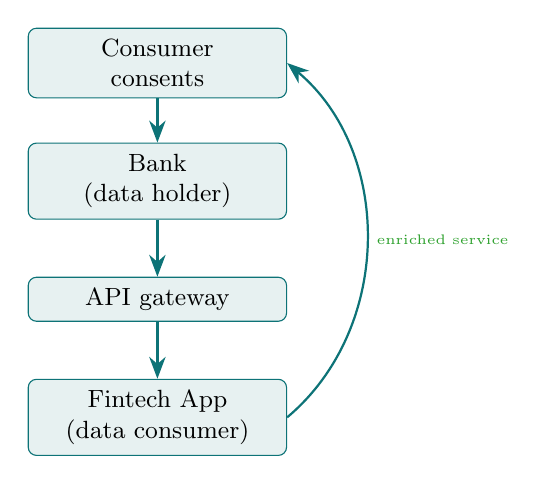
\begin{tikzpicture}[
        box/.style={draw=MLTEAL, fill=MLTEAL!10, rounded corners=3pt,
                    text width=3.0cm, align=center, font=\small, inner sep=4pt},
        arr/.style={-{Stealth[scale=1.2]}, thick, color=MLTEAL}
      ]
        \node[box] (cons) at (0,0)    {Consumer\\consents};
        \node[box] (bank) at (0,-1.5) {Bank\\(data holder)};
        \node[box] (api)  at (0,-3.0) {API gateway};
        \node[box] (app)  at (0,-4.5) {Fintech App\\(data consumer)};
        \draw[arr] (cons) -- (bank);
        \draw[arr] (bank) -- (api);
        \draw[arr] (api)  -- (app);
        \draw[arr] (app.east) to[bend right=50]
              node[right, font=\tiny, text=MLGREEN] {enriched service} (cons.east);
      \end{tikzpicture}
    \end{column}
  \end{columns}
  \bottomnote{Open banking is a \emph{regulatory} phenomenon as much as a technology one. Compliance is the floor; competitive advantage is built above it.}
\end{frame}

\section{Risks and Challenges}

% ---------------------------------------------------------
% Frame 16: Fintech Failure Modes (lighter treatment per spec)
% ---------------------------------------------------------
\begin{frame}{When Fintech Fails -- Four Failure Modes}
  \begin{itemize}
    \item[\textcolor{mlred}{1.}] \textcolor{mlred}{\textbf{Regulatory risk}} \\
      Operating without adequate licences; crossing jurisdictional boundaries without compliance
    \vspace{0.4em}
    \item[\textcolor{mlorange}{2.}] \textcolor{mlorange}{\textbf{Trust risk}} \\
      Data breaches; lack of deposit insurance; unclear complaint resolution pathways
    \vspace{0.4em}
    \item[\textcolor{mlblue}{3.}] \textcolor{mlblue}{\textbf{Scalability risk}} \\
      Customer acquisition costs exceed lifetime value; unit economics that never work at scale
    \vspace{0.4em}
    \item[\textcolor{mlpurple}{4.}] \textcolor{mlpurple}{\textbf{Systemic risk}} \\
      Fintech becomes ``too connected to fail''; concentration in a small number of cloud providers
  \end{itemize}
  \vspace{0.3em}
  \begin{block}{}
    Fintech disruption is not risk-free. The question is whether fintech creates \textbf{new risks} or merely \textbf{redistributes old ones}.
  \end{block}
  \bottomnote{See L04 (RegTech \& Regulation) for detailed analysis of regulatory failure modes and consumer protection frameworks.}
\end{frame}

% ---------------------------------------------------------
% Frame 17: The Consumer Protection Challenge
% ---------------------------------------------------------
\begin{frame}{The Consumer Protection Challenge}
  \begin{columns}[T]
    \begin{column}{0.50\textwidth}
      \textcolor{mlpurple}{\textbf{The regulatory gap:}}
      \vspace{0.4em}

      Traditional banks are \textbf{regulated, insured, and supervised}. Fintech companies often operate between banking law and technology law -- in the gaps that regulators have not yet filled.
      \vspace{0.5em}

      \begin{alertblock}{Core Tension}
        Innovation without consumer protection is not progress -- it is \textcolor{mlred}{\textbf{risk transfer}} from institutions to individuals.
      \end{alertblock}
    \end{column}
    \begin{column}{0.46\textwidth}
      \textcolor{mlblue}{\textbf{Key consumer concerns:}}
      \begin{itemize}
        \item Deposit insurance gaps for neobank customers
        \item Data privacy vulnerabilities via third-party APIs
        \item Algorithmic bias in lending and credit scoring
        \item Cross-border enforcement difficulties
        \item Lack of clear recourse when things go wrong
      \end{itemize}
    \end{column}
  \end{columns}
  \bottomnote{This tension between innovation and protection is the central theme of L04 (Fintech Security and Regulation).}
\end{frame}

\section{Global Landscape}

% ---------------------------------------------------------
% Frame 18: Fintech Around the World (SOLUTION -- evidence)
% ---------------------------------------------------------
\begin{frame}{Fintech Around the World -- Regional Patterns}
  \begin{center}
    \includegraphics[width=0.88\textwidth]{figures/09_fintech_impact_comparison/chart.pdf}
  \end{center}
  \vspace{-0.3em}
  \begin{itemize}
    \item Asia-Pacific and Africa lead in \textbf{mobile payments}; the West leads in digital lending
    \item \textcolor{mlpurple}{\textbf{Leapfrog effect:}} weak traditional infrastructure $\Rightarrow$ faster fintech adoption
  \end{itemize}
  \bottomnote{The most transformative fintech innovations (M-Pesa, Alipay, PIX) emerged outside the US and Europe. Fintech is not a Western phenomenon.}
\end{frame}

% ---------------------------------------------------------
% Frame 19: Key Trends
% ---------------------------------------------------------
\begin{frame}{Five Trends Reshaping Fintech Today}
  \begin{enumerate}
    \item \textcolor{mlpurple}{\textbf{Embedded finance}} \\
      Financial services integrated into non-financial platforms -- ride-sharing with payments, e-commerce with lending
    \vspace{0.25em}
    \item \textcolor{mlblue}{\textbf{Neobanks}} \\
      Digital-only banks challenging incumbents on user experience and fees, without branches
    \vspace{0.25em}
    \item \textcolor{mlteal}{\textbf{Decentralised finance (DeFi)}} \\
      Financial services built on blockchain, removing traditional intermediaries
    \vspace{0.25em}
    \item \textcolor{mlorange}{\textbf{Super-apps}} \\
      Single platforms combining messaging, payments, shopping, and banking (WeChat, Grab, Gojek)
    \vspace{0.25em}
    \item \textcolor{mlgreen}{\textbf{Sustainable fintech}} \\
      Green bonds, ESG scoring engines, carbon-tracking financial products
  \end{enumerate}
  \bottomnote{Each of these trends is both an opportunity and a threat. Lectures 3--7 examine them in depth. Today we establish the landscape.}
\end{frame}

\section{Stakeholder Impact}

% ---------------------------------------------------------
% Frame 20: Stakeholder Impact (SOLUTION)
% ---------------------------------------------------------
\begin{frame}{Who Wins and Who Loses? Stakeholder Analysis}
  \begin{columns}[T]
    \begin{column}{0.47\textwidth}
      \textcolor{mlgreen}{\textbf{Potential winners:}}
      \begin{itemize}
        \item \textbf{Consumers} -- more choice, lower fees, mobile-first access
        \item \textbf{Fintech startups} -- growth opportunity in large addressable markets
        \item \textbf{Regulators} -- better data via APIs; RegTech improves compliance
        \item \textbf{Unbanked populations} -- mobile money, micro-lending, remittances
      \end{itemize}
    \end{column}
    \begin{column}{0.47\textwidth}
      \textcolor{mlred}{\textbf{Potential losers:}}
      \begin{itemize}
        \item \textbf{Incumbent banks} -- margin compression, forced technology investment
        \item \textbf{Bank employees} -- automation of routine tasks
        \item \textbf{Consumers (risk)} -- less protection in unregulated gaps
        \item \textbf{Society} -- digital divide; those without smartphones excluded
      \end{itemize}
    \end{column}
  \end{columns}
  \vspace{0.4em}
  \begin{block}{}
    Fintech is \textcolor{mlpurple}{\textbf{not zero-sum}}. Both consumers and institutions can benefit -- but the benefits are not evenly distributed.
  \end{block}
  \bottomnote{Financial inclusion -- serving the unbanked and underbanked -- is examined in detail in L02 (Fintech Ecosystem).}
\end{frame}

% ---------------------------------------------------------
% Frame 21: The Financial Inclusion Promise
% ---------------------------------------------------------
\begin{frame}{The Financial Inclusion Promise}
  \begin{columns}[T]
    \begin{column}{0.55\textwidth}
      \textcolor{mlpurple}{\textbf{The scale of the problem:}}
      \vspace{0.3em}

      Over \textcolor{mlpurple}{\textbf{1.7 billion adults}} globally lack access to formal financial services. They cannot save securely, borrow affordably, or send money cheaply.

      \vspace{0.5em}
      \textcolor{mlblue}{\textbf{How fintech helps:}}
      \begin{itemize}
        \item \textbf{Mobile money} serving unbanked populations (M-Pesa model)
        \item \textbf{Alternative credit scoring} using non-traditional data
        \item \textbf{Micro-investing} lowering entry barriers to wealth-building
        \item \textbf{Remittance cost reduction} for migrant workers
      \end{itemize}
    \end{column}
    \begin{column}{0.41\textwidth}
      \begin{block}{The Inclusion Test}
        If fintech only serves the \emph{already-served}, it is \textbf{optimisation}, not \textbf{transformation}.\\[0.5em]
        Inclusion is the test of genuine impact.
      \end{block}
      \vspace{0.5em}
      \textcolor{mlgray}{\small M-Pesa (Kenya, 2007) remains the canonical example. It brought formal financial services to millions who had never had a bank account -- using mobile phones, not branches.}
    \end{column}
  \end{columns}
  \bottomnote{M-Pesa is the most studied case of fintech-driven financial inclusion. See L02 for the full discussion of the leapfrog effect in developing markets.}
\end{frame}

\section{Evaluation Framework}

% ---------------------------------------------------------
% Frame 22: Five Questions (PRACTICE -- evaluation tool)
% ---------------------------------------------------------
\begin{frame}{Five Questions That Reveal Any Fintech's True Strategy}
  \begin{enumerate}
    \item \textcolor{mlpurple}{\textbf{Who is the customer?}} \\
      Consumer, SME, enterprise, or another fintech?
    \vspace{0.3em}
    \item \textcolor{mlblue}{\textbf{What part of the value chain does it attack?}} \\
      Origination, distribution, servicing, or infrastructure?
    \vspace{0.3em}
    \item \textcolor{mlgreen}{\textbf{How does it make money?}} \\
      Transaction fees, subscription, data monetisation, or float?
    \vspace{0.3em}
    \item \textcolor{mlorange}{\textbf{What is its regulatory position?}} \\
      Licensed, partnered, or operating in a gap?
    \vspace{0.3em}
    \item \textcolor{mlteal}{\textbf{Does it create or capture value?}} \\
      Building new markets, or taking share from incumbents?
  \end{enumerate}
  \vspace{0.2em}
  \begin{block}{}
    These five questions work for \textbf{any} fintech company you encounter -- in this course, in the news, or in your career.
  \end{block}
  \bottomnote{Apply these questions to a fintech you use. You will use this framework in the Workshop C evaluation exercise on Day 5.}
\end{frame}

% ---------------------------------------------------------
% Frame 23: The Central Tension Revisited
% ---------------------------------------------------------
\begin{frame}{The Central Tension Revisited}
  \begin{center}
    \Large
    \textcolor{mlteal}{\textbf{``Technology is reshaping finance -- but the outcome depends on design choices.''}}
  \end{center}

  \vspace{0.5em}
  \begin{itemize}
    \item Will fintech \textbf{replace institutions} or strengthen them?
    \item Will it \textbf{include the excluded} or serve only the already-served?
    \item Will it create \textbf{resilience} or fragility?
  \end{itemize}

  \vspace{0.5em}
  \begin{block}{}
    These are not technology questions. They are \textcolor{mlpurple}{\textbf{governance, regulation, and strategy questions}}. This course gives you the tools to answer them.
  \end{block}

  \vspace{0.3em}
  \textcolor{mlgray}{\small Fintech is not a technology story. It is a governance story told in the language of technology.}
  \bottomnote{This course covers: Ecosystem (L02), Payments (L03), Regulation (L04), Wealth Management (L05), Insurance (L06), and Technology (L07).}
\end{frame}

% ---------------------------------------------------------
% Frame 24: What Comes Next
% ---------------------------------------------------------
\begin{frame}{What Comes Next}
  \begin{itemize}
    \item \textcolor{mlpurple}{\textbf{Next: L02 (Fintech Ecosystem)}} \\
      Growth drivers, financial inclusion, trust in fintech, and behavioral dimensions of digital financial services
    \vspace{0.4em}
    \item \textcolor{mlblue}{\textbf{This afternoon:}} L02 begins at 11:30 after the break
    \vspace{0.4em}
    \item \textcolor{mlgreen}{\textbf{Before L02, reflect:}}
      \begin{itemize}
        \item What fintech services do you trust \emph{more} than your bank? Why?
        \item What fintech services do you trust \emph{less}? Why?
      \end{itemize}
  \end{itemize}

  \vspace{0.5em}
  \begin{block}{The Rest of the Course}
    L01 gave you the \textbf{map}. Starting with L02, we explore each \textbf{territory} -- in greater depth, with case studies and live examples.
  \end{block}
  \bottomnote{If you want to read ahead, the course website has all lecture slides and materials available for download.}
\end{frame}

% ============================================================
% ZONE 3: CLOSING
% Frames 25-27 -- Fixed closing sequence
% ============================================================

\section{Closing}

% ---------------------------------------------------------
% Frame 25: Closing Cartoon
% ---------------------------------------------------------
\begin{frame}{The Partnership Imperative}
  \begin{center}
    \includegraphics[width=0.90\textwidth]{figures/12_closing_cartoon/cartoon.pdf}
  \end{center}
  \bottomnote{The collaboration imperative is the most important take-away from this lecture. Neither banks nor fintechs can win alone.}
\end{frame}

% ---------------------------------------------------------
% Frame 26: Key Takeaways
% ---------------------------------------------------------
\begin{frame}{Key Takeaways}
  \begin{enumerate}
    \item \textcolor{mlpurple}{\textbf{Fintech defined:}} Technology-enabled innovation that creates new financial products, processes, or business models
    \vspace{0.2em}
    \item \textcolor{mlblue}{\textbf{Historical arc:}} From credit cards (1950s) through online banking (1990s) to embedded finance (2020s) -- each wave built on the last
    \vspace{0.2em}
    \item \textcolor{mlgreen}{\textbf{Crisis catalyst:}} The 2008 crisis eroded trust, opened regulatory space, and released talent -- creating the conditions for fintech's growth
    \vspace{0.2em}
    \item \textcolor{mlorange}{\textbf{Unbundling:}} Fintech companies attack specific layers of the banking value chain, not the entire bank
    \vspace{0.2em}
    \item \textcolor{mlteal}{\textbf{Collaboration spectrum:}} Partnership, acquisition, white-label, and open banking each carry distinct trade-offs
    \vspace{0.2em}
    \item \textcolor{mlred}{\textbf{Global variation:}} Adoption is highest where traditional infrastructure is weakest -- the leapfrog effect
    \vspace{0.2em}
    \item \textcolor{mlpurple}{\textbf{Evaluation tool:}} Five questions (customer, value chain, revenue, regulation, value creation) reveal any fintech's true strategy
  \end{enumerate}
  \bottomnote{Review question: Which collaboration model would you recommend for a mid-sized European bank entering mobile payments? Why?}
\end{frame}

% ---------------------------------------------------------
% Frame 27: Summary and Vocabulary
% ---------------------------------------------------------
\begin{frame}{Summary and Key Vocabulary}
  \begin{block}{Lecture Summary}
    Fintech is the application of technology to financial services, driven by the convergence of eroded trust,
    enabling technology, and regulatory change after 2008. Banks and fintech companies are increasingly choosing
    \textbf{collaboration over competition}, through models ranging from partnerships to open banking APIs.
    The key question is not whether fintech will transform finance, but \textcolor{mlpurple}{\textbf{how the benefits
    and risks will be distributed}} across stakeholders.
  \end{block}
  \vspace{0.4em}
  \begin{multicols}{2}
    \small
    \begin{itemize}
      \item \textbf{Fintech}
      \item \textbf{Neobank}
      \item \textbf{Open Banking}
      \item \textbf{Embedded Finance}
      \item \textbf{Unbundling}
      \item \textbf{Banking-as-a-Service (BaaS)}
      \item \textbf{RegTech}
      \item \textbf{Financial Inclusion}
    \end{itemize}
  \end{multicols}
  \vspace{0.3em}
  \textcolor{mlgray}{\small \textbf{Next lecture:} Fintech Ecosystem -- growth drivers, financial inclusion, trust, and behavioural economics. L02 begins this afternoon at 11:30.}
  \bottomnote{Bring your phone app count from the Frame 5 exercise to the L02 opening discussion.}
\end{frame}

\end{document}
